\documentclass[a4paper]{article}
\usepackage[utf8]{inputenc}
\usepackage[T1]{fontenc}
\usepackage[french]{babel}
\usepackage{graphicx}
\usepackage{algorithmeUTF8}
\usepackage[left=3cm,right=3cm,top=3cm,bottom=3cm]{geometry}
\newcommand{\noun}[1]{\textsc{#1}}

\title{Projet Ruzzle}
\author{Nina \noun{Lardiere}, Yves \noun{Le Guennec}, Simon \noun{Lebeaud}, Tanguy \noun{Leclerc}}
\date{Novembre 2018}

\begin{document}
	\maketitle
	%\newpage
	%\tableofcontents
	\section{Analyse}
		\subsection{Les TAD}
			\begin{tad}
  \tadNom{Case}
  \tadDependances{A..Z,\naturelNonNul,Bonus}
  \begin{tadOperations}{obtenirNbPoints}%nom de l'opération le plus long
    \tadOperation{creerCase}{}{\tadUnParam{Case}}
    \tadOperation{fixerLettre}{\tadDeuxParams{Case}{A..Z}}{\tadUnParam{Case}}
    \tadOperation{fixerNbPoints}{\tadDeuxParams{Case}{\naturelNonNul}}{\tadUnParam{Case}}
    \tadOperation{fixerBonus}{\tadDeuxParams{Case}{Bonus}}{\tadUnParam{Case}}
    \tadOperation{obtenirLettre}{\tadUnParam{Case}}{\tadUnParam{A..Z}}
    \tadOperation{obtenirNbPoints}{\tadUnParam{Case}}{\tadUnParam{\naturelNonNul}}
    \tadOperation{obtenirBonus}{\tadUnParam{Case}}{\tadUnParam{Bonus}}
  \end{tadOperations}
  \begin{tadAxiomes}
    \tadAxiome{obtenirLettre(creerCase())='A'}
    \tadAxiome{obtenirNbPoints(creerCase())=1}
    \tadAxiome{obtenirBonus(creerCase())="\textvisiblespace\textvisiblespace"}
    \tadAxiome{obtenirLettre(fixerLettre(uneCase,uneLettre))=uneLettre}
    \tadAxiome{obtenirBonus(fixerBonus(uneCase,leBonus))=leBonus}
    \tadAxiome{obtenirNbPoints(fixerNbPoints(uneCase,nbPoints))=nbPoints}
  \end{tadAxiomes}
\end{tad}
\medskip

\begin{tad}
  \tadNom{Grille}
  \tadDependances{Case,\booleen,1..4}
  \begin{tadOperations}{DebutUtilisation}%nom de l'opération le plus long
      \tadOperation{creerGrille}{}{\tadUnParam{Grille}}
      \tadOperation{obtenirCase}{\tadTroisParams{Grille}{1..4}{1..4}}{\tadUnParam{Case}}
      \tadOperation{fixerCase}{\tadQuatreParams{Grille}{Case}{1..4}{1..4}}{\tadUnParam{Grille}}
      \tadOperation{estUtilisee}{\tadTroisParams{Grille}{1..4}{1..4}}{\tadUnParam{\booleen}}
      \tadOperation{debutUtilisation}{\tadTroisParams{Grille}{1..4}{1..4}}{\tadUnParam{Grille}}
      \tadOperation{finUtilisation}{\tadTroisParams{Grille}{1..4}{1..4}}{\tadUnParam{Grille}}
  \end{tadOperations}
  \begin{tadAxiomes}
    \tadAxiome{obtenirCase(creerGrille,x,y)=creerCase()}
    \tadAxiome{obtenirCase(fixerCase(c,x,y))=c}
    \tadAxiome{estUtilisee(debutUtilisation(g,x,y))=VRAI}
    \tadAxiome{estUtilisee(finUtilisation(g,x,y))=FAUX}
  \end{tadAxiomes}
\end{tad}
\medskip

\begin{tad}
  \tadNom{Mot}
  \tadDependances{Dictionnaire,\chaine,\naturelNonNul,\caractere}
  \begin{tadOperations}{ajouterLettre}%nom de l'opération le plus long
    \tadOperationAvecPreconditions{chaineEnMot}{\tadDeuxParams{Dictionnaire}{\chaine}}{\tadUnParam{Mot}}
    \tadOperation{motEnChaine}{\tadUnParam{Mot}}{\tadUnParam{\chaine}}
    \tadOperation{longueur}{\tadUnParam{Mot}}{\tadUnParam{\naturelNonNul}}
    \tadOperationAvecPreconditions{ajouterLettre}{\tadTroisParams{Dictionnaire}{Mot}{\caractere}}{\tadUnParam{Mot}}
    \tadOperationAvecPreconditions{retirerLettre}{\tadUnParam{Mot}}{\tadUnParam{Mot}}
  \end{tadOperations}
  \begin{tadPreconditions}{retirerLettre}
    \tadPrecondition{chaineEnMot}{estUnPrefixe(dico,chaine) ET longueur(chaine)$\geq$1}
    \tadPrecondition{ajouterLettre}{estUnPrefixe(dico,motEnChaine(unMot)+lettre)}
    \tadPrecondition{retirerLettre}{longueur(unMot) $\geq$ 2}
   \end{tadPreconditions}
   \begin{tadAxiomes}
     \tadAxiome{motEnChaine(chaineEnMot(dico,uneChaine))=uneChaine}
     \tadAxiome{motEnChaine(ajouterLettre(dico,unMot,lettre))=motEnChaine(unMot)+lettre}
     \tadAxiome{longueur(ajouterLettre(dico,unMot,lettre))=longueur(unMot)+1}
     \tadAxiome{longueur(retirerLettre(unMot))=longueur(unMot)-1}
   \end{tadAxiomes}
\end{tad}
\medskip

\begin{tad}
  \tadNom{Dictionnaire}
  \tadDependances{Mot,\chaine,Fichier,\booleen}
  \begin{tadOperations}{obtenirLettresSuivantes}%nom de l'opération le plus long
    \tadOperation{creerDictionnaire}{\tadUnParam{Ensemble<\chaine>}}{\tadUnParam{Dictionnaire}}
    \tadOperation{ajouterMot}{\tadDeuxParams{Dictionnaire}{\chaine}}{\tadUnParam{Dictionnaire}}
    % pas nécessaire pour le Ruzzle, tous les mots étant contenus dans le fichier utilisé par creerDictionnaire
    \tadOperationAvecPreconditions{supprimerMot}{\tadDeuxParams{Dictionnaire}{Mot}}{\tadUnParam{Dictionnaire}}
   % pas nécessaire pour le Ruzzle
    \tadOperation{estUnPrefixe}{\tadDeuxParams{Dictionnaire}{\chaine}}{\tadUnParam{\booleen}}
    \tadOperation{estUnMot}{\tadDeuxParams{Dictionnaire}{Mot}}{\tadUnParam{\booleen}}
    \tadOperation{obtenirLettresSuivantes}{\tadDeuxParams{Dictionnaire}{Mot}}{\tadUnParam{Ensemble<A..Z>}}
    \tadOperation{sauvegarder}{\tadUnParam{Dictionnaire}}{\tadUnParam{Fichier}}
    \tadOperation{charger}{\tadUnParam{Fichier}}{\tadDeuxParams{Dictionnaire}{\booleen}}
  \end{tadOperations}
  \begin{tadPreconditions}{retirerLettre}
    \tadPrecondition{supprimerMot}{estUnMot(motASupprimer)}
   \end{tadPreconditions}
  \begin{tadSemantiques}{obtenirLettresSuivantes}
    \tadSemantique{creerDictionnaire}{création d'un dictionnaire à partir d'une suite de mots}
    \tadSemantique{ajouterMot}{ajout d'un mot dans le dictionnaire}
    \tadSemantique{supprimerMot}{suppression d'un mot du dictionnaire}
    \tadSemantique{estUnPrefixe}{indique si la suite de caractères est le début d'un mot du dictionnaire}
    \tadSemantique{estUnMot}{indique si le préfixe est un mot complet}
    \tadSemantique{obtenirLettresSuivantes}{indique, pour un préfixe donné, toutes les lettres qui peuvent suivre le préfixe pour former un nouveau préfixe}
    \tadSemantique{sauvegarder}{sauvegarde le dictionnaire dans un fichier}
    \tadSemantique{charger}{charge le dictionnaire à partir d'un fichier préalablement généré par l'opération sauvegarder}
  \end{tadSemantiques}
\end{tad}
\medskip

\begin{tad}
  \tadNom{CasesContigues}
  \tadDependances{Case,\naturel,\chaine}
  \begin{tadOperations}{CasesContiguesEnChaine}
    \tadOperation{creerCasesContigues}{}{\tadUnParam{CasesContigues}}
    \tadOperation{ajouterCase}{\tadDeuxParams{CasesContigues}{Case}}{\tadUnParam{CasesContigues}}
    \tadOperationAvecPreconditions{supprimerCase}{\tadUnParam{CasesContigues}}{\tadUnParam{CasesContigues}}
    \tadOperation{nbCasesContigues}{\tadUnParam{CasesContigues}}{\tadUnParam{\naturel}}
    \tadOperation{casesContiguesEnChaine}{\tadUnParam{CasesContigues}}{\tadUnParam{\chaine}}
  \end{tadOperations}
  \begin{tadPreconditions}{supprimerCase}
     \tadPrecondition{supprimerCase}{nbCasesContigues(suiteCases) $>$ 0}
  \end{tadPreconditions}
  \begin{tadAxiomes}
    \tadAxiome{supprimerCase(ajouterCase(suiteCases,uneCase))=uneCase}
    \tadAxiome{nbCasesContigues(creerCasesContigues())=0}
  \end{tadAxiomes}
\end{tad}


		\subsection{Analyse descendante}
			voir Figure \ref{fig:AD}
			\begin{figure}
				\centering 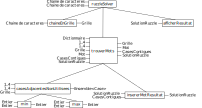
\includegraphics[width=1\textwidth]{./analyseDescendante}
				\caption{\label{fig:AD}Analyse descendante}
			\end{figure}

 \section{Conception préliminaire}
		\subsection{Signatures des fonctions et procédures des TAD}
			\paragraph{Case}
\begin{algorithme}
  \signaturefonction
  {creerCase}{}{Case}

  \signatureprocedure
  {fixerLettre}{\paramEntreeSortie{c : Case}; \paramEntree{uneLettre : A..Z}}

  \signatureprocedure
  {fixerNbPoints}{\paramEntreeSortie{c : Case}; \paramEntree{nbPoints : \naturelNonNul}}

  \signatureprocedure
  {fixerBonus}{\paramEntreeSortie{c : Case}; \paramEntree{bonus : Bonus}}

  \signaturefonction
  {obtenirLettre}{c : Case}{A..Z}

  \signaturefonction
  {obtenirNbPoints}{c : Case}{\naturelNonNul}

  \signaturefonction
  {obtenirBonus}{c : Case}{Bonus}
\end{algorithme}

\paragraph{Grille}
\begin{algorithme}
  \signaturefonction
  {creerGrille}{}{Grille}

  \signaturefonction
  {obtenirCase}{g : Grille ; coordX, coordY : 1..4 }{Case}

  \signatureprocedure
  {fixerCase}{\paramEntreeSortie{g : Grille}; \paramEntree{c :Case ; coordX, coordY : 1..4}}

  \signaturefonction
  {estUtilisee}{g : Grille ; coordX, coordY : 1..4}{\booleen}

  \signatureprocedure
  {debutUtilisation}{\paramEntreeSortie{g : Grille}; \paramEntree{xUtilisee, yUtilisee : 1..4}}

  \signatureprocedure
  {finUtilisation}{\paramEntreeSortie{g : Grille}; \paramEntree{xUtilisee, yUtilisee : 1..4}}

\end{algorithme}

			\paragraph{CasesContigues}
\begin{algorithme}
	\signaturefonction{creerCasesContigues}{}{CasesContigues}
	\signatureprocedure{ajouterCase}{\paramEntreeSortie{suiteCases : CasesContigues} \paramSortie{uneCase : Case}}
	\signatureProcedureAvecPreconditions {supprimerCase}{\paramEntreeSortie{suiteCases : CasesContigues}}{nbCasesContigues(suiteCases) $>$ 0}
	\signaturefonction{nbCasesContigues}{suiteCase : CasesContigues}{\naturel}
	\signaturefonction{casesContiguesEnChaine}{suiteCases : CasesContigues}{\chaine}
\end{algorithme}

			\paragraph{Mot}
\begin{algorithme}
  \signatureFonctionAvecPreconditions
  {chaineEnMot}{dico : Dictionnaire ; chaine : \chaine}{Mot}{estUnPrefixe(dico,chaine) ET longueur(chaine)$\geq$1}

  \signaturefonction
  {motEnChaine}{leMot : Mot}{\chaine}

  \signaturefonction
  {longueur}{leMot : Mot}{\naturelNonNul}

  \signatureProcedureAvecPreconditions
  {ajouterLettre}{\paramEntreeSortie{leMot : Mot} \paramEntree{lettre : \caractere; dico : Dictionnaire}}{estUnPrefixe(dico,motEnChaine(leMot)+lettre)}

  \signatureProcedureAvecPreconditions
  {retirerLettre}{\paramEntreeSortie{leMot : Mot}}{longueur(leMot) $\geq$ 2}

\end{algorithme}

			\paragraph{Dictionnaire}
\begin{algorithme}

  \signaturefonction
  {creerDictionnaire}{lesMots : Ensemble<\chaine>}{Dictionnaire}

  \signatureProcedure
  {ajouterMot}{\paramEntreeSortie{dico : Dictionnaire} \paramEntree{leMot : \chaine}}
  % pas nécessaire pour le Ruzzle, tous les mots étant contenus dans le fichier utilisé par creerDictionnaire

  \signatureProcedureAvecPreconditions
  {supprimerMot}{\paramEntreeSortie{dico : Dictionnaire} \paramEntree{motASupprimer : Mot}}{estUnMot(motASupprimer)}

  % pas nécessaire pour le Ruzzle
  \signaturefonction
  {estUnPrefixe}{dico : Dictionnaire ; chaine : \chaine}{\booleen}

  \signaturefonction
  {estUnMot}{dico : Dictionnaire ; prefixe : Mot}{\booleen}

  \signaturefonction
  {obtenirLettresSuivantes}{dico : Dictionnaire ; prefixe : Mot}{Ensemble<A..Z>}

  \signatureProcedure
  {sauvegarder}{\paramEntree{dico : Dictionnaire}}

  \signatureProcedure
  {charger}{\paramEntree{fichier : Fichier} \paramSortie{dico : Dictionnaire ; erreur : \booleen}}

\end{algorithme}


		\subsection{Signatures des fonctions et procédures de l'analyse descendante}

\section{Conception détaillée}
	\begin{algorithme}
  \procedure
    {trouverMots}
    {\paramEntree{posX, posY: 1..4 ; dico: Dictionnaire} \paramEntreeSortie{g: Grille; prefixe: Mot; cheminRuzzle : CasesContigues, resultat: SolutionRuzzle}}
    {lettresPossibles: Ensemble<A..Z>}
    {
      \instruction{debutUtilisation(g,posX,posY)}
      \affecter{lettresPossibles}{obtenirLettresSuivantes(dico,prefixe)}
      \pourChaque{case}{casesAdjacentesNonUtilisees(posX,posY,g)}{
        \sialors{estPresent(obtenirLettre(case),lettresPossibles)}{
          \instruction{ajouterLettre(dico,prefixe,obtenirLettre(case))}
          \instruction{ajouterCase(cheminRuzzle,case)}
          \sialors{estUnMot(prefixe)}{
            \instruction{insererMotResultat(resultat,cheminRuzzle)}
          }
          \instruction{trouverMots(obtenirPosX(case),obtenirPosY(case),dico,g,prefixe,cheminRuzzle,resultat)}
          \instruction{retirerLettre(prefixe)}
          \instruction{supprimerCase(cheminRuzzle)}
        }

      }
      \instruction{finUtilisation(g,posX,posY)}
    }
\end{algorithme}

	\begin{algorithme}
  \fonction
    {casesAdjacentesNonUtilisees}
    {posX, posY : 1..4 ; g : Grille}
    {Ensemble<Case>}
    {x, y, borneMinX, borneMaxX, borneMinY, borneMaxY : 1..4 ; casesAdjacentes : Ensemble<Case>}
    {
      \affecter{borneMinX}{max(1,posX-1)}
      \affecter{borneMaxX}{min(4,posX+1)}
      \affecter{borneMinY}{max(1,posY-1)}
      \affecter{borneMaxY}{min(4,posY+1)}
      \affecter{casesAdjacentes}{ensemble()}
      \pour{y}{borneMinY}{borneMaxY}{}{
        \pour{x}{borneMinX}{borneMaxX}{}{
          \sialors{((x$\ne$posX) OU (y$\ne$posY)) ET non estUtilisee(g,x,y)}{
            \instruction{ajouter(casesAdjacentes,obtenirCase(g,x,y))}
          }
        }
      }
      \retourner{casesAdjacentes}
    }
\end{algorithme}

	\begin{algorithme}
  \procedure
    {ruzzleSolver}
    {\paramEntree{grilleRuzzle, nomFichierDico: \chaine}}
    {g : Grille, dico: Dictionnaire, resultat: solutionRuzzle, initMot : Mot, initChemin : CasesContigues}
    {
      \affecter{g}{chaineEnGrille(grilleRuzzle)}
      \affecter{dico}{charger(nomFichierDico)}
      \affecter{resultat}{creer()}
      \pour{y}{1}{4}{}{
        \pour{x}{1}{4}{}{
          \affecter{initMot}{chaineEnMot(dico,caractereEnChaine(obtenirLettre(obtenirCase(g,x,y))))}
          \affecter{initChemin}{creerCasesContigues()}
          \instruction{ajouterCase(initChemin,obtenirCase(g,x,y))}
          \instruction{trouverMot(x,y,dico,g,initMot,initChemin,resultat)}
        }
      }
      \instruction{afficherResultat(resultat)}
    }
\end{algorithme}

\end{document}
